\documentclass[12pt]{article}
%----------Title & Cover-----------%
\title{Math 347: Fundamental Mathematics}
\author{Lanxiao Hermite Bai}
\date{\today}

%-----------Packeges---------------%
\usepackage{amsmath}
\usepackage{amssymb}
\usepackage{amsfonts}
\usepackage{tocloft}
\usepackage{float}
\usepackage{graphicx}
\usepackage[bookmarks=true]{hyperref}
\usepackage{fancyhdr}
\usepackage{tikz}


%----------Definition & Theorem----%
\newtheorem{definition}{Definition}[subsection]
\newtheorem{theorem}{Theorem}[subsection]
\newtheorem{proposition}{Proposition}[subsection]
\newtheorem{lemma}{Lemma}[subsection]
\newtheorem{corollary}{Corollary}[subsection]
\newtheorem{axiom}{Axiom}[subsection]


\pagestyle{fancy}
\fancyhead[L]{Math 347}
\fancyhead[C]{Note}
\fancyhead[R]{Lanxiao Bai}
\begin{document}
\maketitle
\newpage

\tableofcontents
\newpage

\section{Numbers, sets and functions}
    \subsection{Elementary Inequalities}
    \begin{proposition}
        If $0 < a < b$, then $a^2 < ab < b^2$ and $0 < \sqrt{a} < \sqrt{b}$
    \end{proposition}
    
    \begin{definition}[Absolute Value]
        \[|x| = \left\{ \begin{array}{ll} x & if\ x \geq 0 \\ -x & if\ x \leq 0 \end{array}\right.\]
    \end{definition}
    \begin{proposition}[Triangle Inequality]
        If $x, y \in \mathbb{R}$, $|x+y| \leq |x| 
        + |y|$
    \end{proposition}
    \begin{proposition}[AGM Inequality]
        If $x, y \in \mathbb{R}$, $2xy \leq x^2 + y^2$ and $xy \leq (\frac{x+y}{2})^2$.
    \end{proposition}
    
    \textbf{Proof:}
        Since $(x - y)^2 \geq 0$, $x^2 -2xy + y^2 \geq 0$, when we add $2xy$ to both sides, we have $2xy \leq x^2 + y^2$, when we add $4xy$ on both sides and calculate the square root, we have $xy \leq (\frac{x+y}{2})^2$.
    
    \begin{corollary}
        If $x, y > 0$, $\frac{2xy}{x+y} \leq \sqrt{xy} \leq \frac{x+y}{2}$, equality holds only when $x = y$.\footnote{Arithmetic Mean: $\frac{x+y}{2}$, Geometric Mean: $\sqrt{xy}$, Harmonic Mean: $\frac{2xy}{x+y}$}
    \end{corollary}
    \subsection{Sets}
        \begin{definition}[Set]
            The objects in a \textbf{set} are its \textbf{elements} or \textbf{members}. When x is an element of A, we write $x \in A$, if not, we write $x \notin A$. If $\forall x \in A, x \in B$, then A is a \textbf{subset} of B, and B \textbf{contains} A, we write $A \subseteq B$ or $B \supseteq A$.\footnote{Important sets: $\mathbb{N} \subset \mathbb{Z} \subset \mathbb{Q} \subset \mathbb{R} \subset \mathbb{C}$, in this class $0 \notin \mathbb{N}$.}
        \end{definition}

        \begin{definition}
            Sets $A = B$ if they have the same elements. The \textbf{empty set} $\emptyset$, is the unique set with no elements. A \textbf{proper subset} of a set A is a subset of A that is not A. The \textbf{power set} of a set A is the set of all its subsets.
        \end{definition}

        \begin{definition}
            When $a, b \in \mathbb{Z}$ and $a \leq b$, we use ${a, ..., b}$ to ${i \in Z | a \leq i \leq b}$. When $n \in N$, we write $[n]$ for ${1 ... n}$. The set of even numbers is $\{2k | k \in \mathbb{Z}\}$ and the set of odd numbers is $\{2k + 1 | k \in Z\}$.
        \end{definition}

        \begin{definition}[Intervals]
            When $a, b \in \mathbb{R}$ with $a \leq b$, the \textbf{closed interval} $[a, b]$ is $\{x \in \mathbb{R} | a \leq x \leq b\}$ and the \textbf{open interval} $(a, b)$ is $\{x \in \mathbb{R} | a < x < b\}$.
        \end{definition}

        \begin{definition}
            A \textbf{list} with entries in A consists of elements of A in a specific order, with repetition allowed. A \textbf{k-tuple} is a list with $k$ entries. We write $A^k$ for the set of k-tuples with entries in A.

            An \textbf{ordered pair} is a list with two entries. The \textbf{Cartesian product} of sets S and T, $S \times T = \{(x, y)| x \in S, y \in T\}$
        \end{definition}

        \begin{definition}[Set Operations]
            Let A and B be sets,
            \begin{itemize}
                \item Union $A \cup B = \{x | x \in A\ or\ x \in B\}$
                \item Intersection $A \cap B = \{x | x \in A\ and\ x \in B\}$
                \item Difference $A - B = \{x | x \in A\ and\ x \notin B\}$
                \item Complement $A^c = U - A$
            \end{itemize}
            If $A \cup B = \emptyset$, they are \textbf{disjoint}.
        \end{definition}

        \subsection{Functions}
        \begin{definition}[Function]
            A \textbf{function} $f$ from a set A to a set B assigns to each $a \in A$ a single element $f(a) \in B$, called the \textbf{image} of a under $f$. For a function $f: A \rightarrow B$, A is the \textbf{domain}, B is the \textbf{target}. The \textbf{image} of $f$ is $\{f(a), a \in A\}$.\footnote{A function is called \textbf{well-defined} means that rules assign to each element of A exactly one element, belongling to B.}
        \begin{figure}[H]
            \begin{center}
                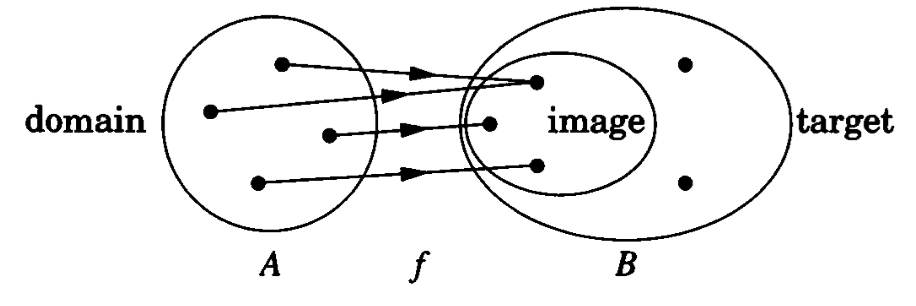
\includegraphics[width=7cm]{./imgs/mapping.png}
                \caption{Mapping}
            \end{center}
        \end{figure}
        \end{definition}
        
        \begin{definition}
            For 2 functions $f$ and $g$, $f = g$ when they have same domain, same targer and $\forall x \in$ domain, $f(x) = g(x)$.
        \end{definition}


        \begin{definition}
            A function is \textbf{real-valued} if its image is a subset of $\mathbb{R}$. If $f$ and $g$ are real-valued functions on A, $f + g$ and $fg$ will be real-valued functions on A defined by $(f+g)(x) = f(x) + g(x)$ and $(fg)(x) = f(x)g(x)$.
        \end{definition}

        \begin{definition}[Polynomial]
            A real \textbf{polynomial} in one variable is a function $f: \mathbb{R} \rightarrow \mathbb{R}$ defined by
            \[f(x) = \sum_{i=0}^k c_ix^i\]
            where k is a nonnegative integer and $c_0, ..., c_k$ are real numbers called the coefficients of $f$. The \textbf{degree} of $f$ is the largest $d$ such that $c_d \neq 0$.
        \end{definition}

        \begin{definition}
            A set $S \subseteq \mathbb{R}$ is \textbf{bounded} if $\exists M \in \mathbb{R}, \forall x \in S, |x| \leq M$, or the set is \textbf{unbounded}.
        \end{definition}
        
        \begin{definition}
            A function is \textbf{increasing} in a certain interval if $\forall x_2 > x_1, f(x_2) > f(x_1)$, \textbf{decreasing} if $f(x_2) < f(x_1)$.
        \end{definition}

\section{Logic and Proofs}
    \subsection{Quantifiers and Logical Statements}
    \begin{definition}[Mathematical Statement]
        A \textbf{mathematical statement} is a statement that can be evaluated to be true or false.
    \end{definition}
    
    \begin{definition}[Quantifier]
        Suppose $P(x)$ is a statement involving  the variable $x$ which can take values in a set S, then:
        \begin{itemize}
            \item \textbf{Universally quantified:} For all $x \in S, P(x)$ is true, denoted as $\forall x \in S$, such that $P(x)$ is true.
            \item \textbf{Existentially quantified:} There exists an $x \in S$ such that $P(x)$ is true, denoted as $\exists x \in S, P(x)$ is true.
        \end{itemize}
    \end{definition}
    
    \begin{definition}[Logical Connectives] Suppose $P$ and $Q$ are mathematical statements,
        \begin{itemize}
            \item Negation(not P): $\neg P$
            \item Conjunction(P and Q): $P \wedge Q$
            \item Disjunction(P or Q): $P \vee Q$
            \item Bicondition(P if \& only if Q): $P \Leftrightarrow Q$
            \item Condition(P implies Q)\footnote{P - \textbf{Hypothesis}, Q - \textbf{Conclusion}, $Q \Rightarrow P$ - \textbf{Converse} It is always true if the hypothesis is false.}: $P \Rightarrow Q$
        \end{itemize}

    \end{definition}
    
    \paragraph{\textbf{Rule of negation:}}
        \begin{itemize}
            \item $\neg [(\forall x) P(x)] \Leftrightarrow (\exists x)(\neg P(x))$
            \item $\neg [(\exists x) P(x)] \Leftrightarrow (\forall x)(\neg P(x))$
        \end{itemize}

\subsection{Methods of proof}
    \paragraph{Direct method of proof:} Assume $P$ and argue via logical decuction that $Q$ is also true ($P \Rightarrow Q$).

    \paragraph{Contrapositive} Assume $\neg Q$ follow deductions and conclude $\neg P$ is true ($\neg Q \Rightarrow \neg P$).
    
    \paragraph{Methods of Contradiction} Assume $p$ and $\neg Q$, follow deductions and obtain a contradiction.
    
    \section{Induction}
    	\subsection{Principle of Induction}
	\begin{definition}
		The set $\mathbb{N}$ of natrual numbers is the intersection of all sets $S \subseteq \mathbb{R}$ that have the following properties:
		\begin{enumerate}
			\item $1 \in S$
			\item If $x \in S$, then $x + 1 \in S$
		\end{enumerate}
	\end{definition}
	
	\begin{theorem}[Principle of Induction]
		$\forall n \in \mathbb{N}$, let $P(n)$ be a mathematical statement. If
		\begin{itemize}
			\item $P(1)$ is true 
			\item $\forall k \in \mathbb{N}, P(k) \Rightarrow P(k+1)$
		\end{itemize}
Then $\forall n \in \mathbb{N}, P(n)$.
	\end{theorem}
	
	\begin{theorem}[Strong Induction]
		$\forall n \in \mathbb{N}$, let $P(n)$ be a mathematical statement. If
		\begin{itemize}
			\item P(1) is true 
			\item $\forall k \geq 2$ and $i < k$, $P(i) \Rightarrow P(k)$ 
		\end{itemize}
		Then $\forall n \in \mathbb{N}, P(n)$.
	\end{theorem}
	
	\section{Bijection and Cardinality}
		\subsection{Representing integers}
		\paragraph{Usual way} Decimal representation:\\
		E.x.\[1735 = 10^3 + 7 \cdot 10^2 + 3 \cdot 10 + 5\]
		\begin{definition}
			Let $q \geq 2$ be a natural number. A \textbf{q-ary expansion} or \textbf{base-q expansion} of n is a list $a_m,\cdots, a_0$ of integers that $a_i \in \{0, 1, 2, \cdots, q-1\}$ such that \[n = \sum_{j = 0}^m a_jq^j\]
			
				We write $(a_m,\cdots, a_0)_{q}$ for base-q expansion.\footnote{When $q = 2$, binary, $n = 3$, ternary.}
		\end{definition}
		
		\begin{theorem}
			$\forall q \in \mathbb{N} \forall n \in \mathbb{N}$, n has a unique q-ary expansion. 
		\end{theorem}
		
		\paragraph{Proof:}
		
		The base case, $n = 1$ is true since $1$ is represented by $a_0 = 1$.
		
		Suppose, $n = k$ is true, then when $n = k + 1$.
		If $a_0 = a_1 = ... = a_m = q - 1$,
		\begin{align}
			&k + 1 = \sum_{j = 0}^m (q - 1)q^j + 1\nonumber\\
			&\phantom{k + 1} = (q - 1)\sum_{j = 0}^m q^j + 1\nonumber\\
			&\phantom{k + 1} = (q - 1)\frac{q^{m+!} - 1}{q - 1} + 1\nonumber\\
			&\phantom{k + 1} = q^{m+1} - 1 + 1 = q^{m+1}\nonumber 
		\end{align}
		
		So $k + 1$ is represented by $a_{m + 1} = 1$, $a_i = 0$ for $i \leq m$ 
		If $a_i$ is the first $a$ that $a \neq q - 1$, then
		\[k + 1 = \sum_{j = 0}^{i - 1}a_j q^j + a_iq^i +  \sum_{j = i + 1}^{m}a_j q^j = \sum_{j = 0}^{i - 1}a_j q^j + (a_j + 1)q^i \]
		
		So we can conclude that $\forall q \in \mathbb{N}, \forall n \in \mathbb{N}$, n has a q-ary expansion.
		
		Suppose an integer $n$ has 2 distinct q-ary expansions
		\[n = \sum_{j = 0}^r a_jq^j\] 
		\[\phantom{n} = \sum_{j = 0}^s b_jq^j\]
		
		According to the definition of polynomial, we have $a_j = b_j$ for all $j \leq m$ which is controversial to the hypothesis. Thus such expansion is unique.
		
		If $r = s = m$,
		Then \[\sum_{j = 0}^m a_jq^j - \sum_{j = 0}^m b_jq^j =  = \sum_{j = 0}^m (a_j - b_j)q^j = 0\]
		
		If $r \neq s$, without losing generality, we can suppose that $r > s$, then
		\[\sum_{j = 0}^r a_jq^j - \sum_{j = 0}^s b_jq^j = \sum_{j = 0}^s (a_j - b_j)q^j  + \sum_{j = s + 1}^r b_jq^j = 0\]
		
		According to the definition of polynomial, we have $s \leq a_j = b_j$ for all $j \leq s$ and $b_j = 0$ for all $s\leq j \leq r$, which is controversial to the hypothesis. Thus such expansion is unique.
		
		So we can conclude that $\forall q \in \mathbb{N}, \forall n \in \mathbb{N}$, n has a unique q-ary expansion.
		\subsection{Bijection}
		
		\begin{definition}
			A function $f : A \rightarrow B$ is a \textbf{bijection} if $\forall b \in B, \exists$ exactly one $x \in A$ such that $f(x) = b$.\footnote{Alternative terminology: one-to-one correspondence}
				\footnote{$f$ is a bijection if and only if $f$ is both injective and surjective.}
		\end{definition}
		
		\begin{definition}
			Power set of a set S is the set that is formed by all S's subsets.
		\end{definition}
		
		\begin{definition}
			If $f : a \rightarrow b$ is a bijection that $f(a) = b$. The inverse of $f$, $f^{-1}: B \rightarrow A$ is $f(b) = a$. The inverse of a bijection is a bijection.
		\end{definition}
		\subsection{Cardinality}
		
			\begin{definition}
				The cardinality of a set A is the number of elements of the set. Denote as $|A|$.
			\end{definition}
			
			\begin{definition}
				A set $A$ is finite if there is a bijection $f: A \rightarrow [n]$ for some $n \in \mathbb{N}$
			\end{definition}
			
			\begin{proposition}
				If two set $A$ and $B$ are disjoint, $|A| \cup |B| = |A + B|$.
			\end{proposition}
			
			\begin{corollary}
				\[|A \cup |B| = |A| + |B| - |A \cap B|\]
			\end{corollary}
			
			\begin{definition}
				If a set infinite if it is not finite. If there is a bijection $f : A \rightarrow \mathbb{N}$, then A is \textbf{countably infinite} or it is \textbf{uncountably infinite}.
			\end{definition}
			
			\begin{definition}
				$|A| = |B|$ if there is a bijection $f : A \rightarrow B$.
			\end{definition}
	\section{The Real Numbers}
		\paragraph{Assumption} 
		\begin{itemize}
			\item $\mathbb{Q} \subseteq \mathbb{R}$
			\item $\mathbb{R}$ is a \textbf{field}, which means it's legal to:
					\begin{itemize}
						\item add / subtract
						\item multiply
						\item divide by nonzero real number
						\item associativity
						\item commutativity
						\item distributivity  
					\end{itemize}
			\item $\mathbb{R}$ has an ordering
			\item $\mathbb{R}$ satisfies the completeness axiom
		\end{itemize}
		\subsection{Completeness Axiom}
		
		\begin{definition}
			Let $S \subseteq \mathbb{R}$. A number $\alpha \in \mathbb{R}$ is an \textbf{least upper bound} or \textbf{supremum} of $S$ if $S$ has no upper bound less than $\alpha$. $\beta \in \mathbb{R}$ is an \textbf{greatest lower bound} or \textbf{infimum} of $S$ if $S$ has no lower bound larger than $\beta$.\footnote{Notation: $\mathrm{Sup}(S) = $ supremum of $S$, $\mathrm{inf}(S) =$ infimum of $S$}
		\end{definition}
		
		\begin{axiom}[Completeness Axiom]
			Every nonempty subset of $\mathbb{R}$ that has an upper bound has a least upper bound.	
		\end{axiom}
		
		\begin{theorem}[Archimedean Property]
			Given any positive real numbers $a, b$ there exists $n \in \mathbb{N}$ such that $na > b$.
			
			Equivalently, $\mathbb{N} \subseteq \mathbb{R}$ is not upper bounded.
		\end{theorem}
		
		\subsection{Limits and Continuity}
		
		\begin{definition}[Limit]
			Let $(a_n)$ be a sequence of real numbers, we say that $(a_n)$ \textbf{converges} to $L \in \mathbb{R}$ provided that given an $\varepsilon > 0$, $\exists N \in \mathbb{N}$ such that
			\[|a_n - L| < \varepsilon\] 
			for every $n \geq N$.\footnote{Notation: $(a_n)$ converges to L $\equiv \lim_{n\rightarrow\infty}a_n = L \equiv \lim a_n = L \equiv a_n \rightarrow L$.}
		\end{definition}
		
		\paragraph{e.g.1}
			\subparagraph{Proof:}
		The sequence $a_n = \frac{1}{n}$ converges to $0$.
		
		Let $\varepsilon > 0$ be given. There is $N \in \mathbb{N}$ so that \[\frac{1}{\varepsilon} < N\]
		so $\varepsilon > \frac{1}{N}$. Then $\forall n \geq N$ we have
		\[|a_N - 0| = |\frac{1}{n}| = \frac{1}{n} \leq \frac{1}{N} < \varepsilon\]
		$\blacksquare$
		
		\begin{definition}
			If $(a_n), (b_n)$ are sequences. Assume that $a_n \rightarrow 0$. If
				\[|b_n - L| \leq |a_n|\]
			Then
				\[b_n \rightarrow L\]
		\end{definition}
		\paragraph{Terminology:} Say $(a_n)$ is convergent if it converges to some $L \in \mathbb{R}$.
		
		\begin{proposition}
			A convergent sequence has a unique limit.
		\end{proposition}
		
		\begin{proposition}
			Let $S \subseteq \mathbb{R}$ be a subset, then $\mathrm(S) = \alpha \Leftrightarrow \exists (a_n)$ with $a_n \in S$ and $a_n \rightarrow \alpha$.
		\end{proposition}
		
		\begin{definition}
			A sequence is \textbf{monotone} if it is either nondecreasing($n \geq m \Rightarrow a_n \geq a_m$) or nonincreasing($n \leq m \Rightarrow a_n \leq a_m$)
		\end{definition}
		
		\begin{theorem}[Monotone Convergence Theorem]
			If $(a_n)$ is a bounded monotone sequence, then it converges. If $(a_n)$ is bounded nondecreasing, then $\lim_{x \rightarrow \infty} a_n = \mathrm{Sup}(a_n)$. If $(a_n)$ is bounded nonincreasing, then $\lim_{x \rightarrow \infty} = \mathrm{Inf}(a_n)$
		\end{theorem}
		\begin{lemma}
			If $a_n \leq M \forall a \in \mathbb{N}$, then if $a_n \rightarrow L$ then $L \leq M$.
		\end{lemma}
		
		\begin{proposition}
			If $(a_n)$ is nonincreasing, $(b_n)$ is nondecreasing and if \[a_n - b_n \rightarrow 0\]
			then both $a_n$ and $b_n$ converge and have the same limit.
		\end{proposition}
		
		\begin{lemma}
			If $a_n \rightarrow L$, then $a_n^2 \rightarrow L^2$.
		\end{lemma}
		
		\begin{theorem}
			$\sqrt{x} \in \mathbb{R}$ if $x \geq 0$.
		\end{theorem}
		
		\subsection{K-ary expansion and discountability}
			\begin{definition}
				The \textbf{canonical k-ary expansion} of $\alpha$ is the sequence $(l_n)$ defined by $l_n = $ largest multiple of $\frac{1}{k^n}$ such that $l_n \leq \alpha$.
			\end{definition}
			
			\begin{theorem}
				Let $k \in \mathbb{N}, k\geq 2$, then
				\begin{itemize}
					\item $\forall \alpha \in [0, 1)$ has a canonical k-ary expansion
					\item Every k-ary expansion represent a real number in $[0, 1)$. 
				\end{itemize}
			\end{theorem}
			
			\begin{theorem}[Cantor]
				$\mathbb{R}$ is uncountable.
			\end{theorem}
			
			\begin{lemma}
				If a set $S$ contains an uncountable subset, then $S$ is uncountable.
			\end{lemma}
			
			
			\section{Series and Sequences}
			\subsection{Limits}
			\begin{theorem} Let $(S_n), (T_n)$ be sequences, $\lambda \in \mathbb{R}$, then
				\begin{itemize}
					\item \[\lambda \lim S_n = \lim \lambda S_n\]
					\item \[\lim S_n \pm \lim T_n = \lim (S_n \pm T_n)\]
					\item \[\lim S_n \cdot \lim T_n = \lim (S_n \cdot T_n)\]
					\item \[\lim \frac{1}{S_n} = \frac{1}{\lim S_n}\]
				\end{itemize}
			\end{theorem}
			
			\begin{lemma}
				If $(a_n)$ is convergent, then it is bounded.
			\end{lemma}
			
			\begin{proposition}
				Suppose $(a_n)$ is a sequence such that $\frac{a_{n+1}}{a_n}$ converges to a number $0 \leq x <1$. Then $\lim a_n = 0$. 
			\end{proposition}
			
			\begin{theorem}[Squeeze Theorem]
				Suppose $a_n \leq b_n \leq c_n$ for all $n$. Then if $\lim a_n = L, \lim c_n = L$, then $\lim b_n = L$.
			\end{theorem}
			
			\subsection{Cauchy Sequence}
			\begin{definition}
				A sequence is said to be Cauchy provided given any $\varepsilon > 0$ there is $N \in \mathbb{N}$ such that for all $n, m > N\in \mathbb{N}$
					\[|a_n - a_m| < \varepsilon\]
			\end{definition}
			
			\begin{proposition}
				Any convergent sequence is a Cauchy sequence.
			\end{proposition}
			
			\begin{lemma}
				Every Cauchy sequences is bounded.
			\end{lemma}
			
			\subsection{Infinite Series}
			\begin{definition}
				An \textbf{infinite series} is an infinite summation $\sum_{k = 1}^{\infty}a_k$. The sequence is \textbf{partial sums} is $S_n = \sum_{k = 1}^n a_k$. Say that $\sum_{k = 1}^{\infty} a_k$ converges if $\lim_{n \rightarrow \infty} S_n$ exists.
			\end{definition}
			\begin{theorem}
				The geometric theories
				\[\sum_{k=0}^{\infty}x^k\]
				converges to \[\frac{1}{1 - x}\] if $|x| < 1$ and diverges otherwise.
			\end{theorem}
			
			\paragraph{Remark:} If $(a_k) \rightarrow L \neq 0$, then $\sum_{k = 1}^{\infty} a_k$ diverges.
			\begin{proposition}[Harmonic Series]
				\[\sum_{k = 1}^{\infty} 1/k\] diverges.
			\end{proposition}
			\begin{lemma}
				If $\sum_{k = 1}^{\infty} a_k$ converges, then $a_k \rightarrow 0$.
			\end{lemma}
			
			\begin{proposition}[Comparison Test]
				Suppose that $c_n \geq 0$ for all n. If \[\sum_{n = 1}^{\infty}c_n\] converges and \[|a_n| \leq c_n\] for all $n$, then \[\sum_{n = 1}^{\infty} a_n\] converges.
				
				If \[\sum_{n = 1}^{\infty}c_n\] diverges to $\infty$, then if $a_n \geq c_n$ for all $n$, \[\sum_{n = 1}^{\infty} a_n\] diverges.
			\end{proposition}
			
			\begin{corollary}
				If $\sum |a_n|$ converges then $\sum a_n$ converges as well.
			\end{corollary}
			
			\begin{proposition}
				The sequence $\sum \frac{1}{n^p}$ converges if $p > 1$ and diverges if $p \leq 1$.
			\end{proposition}
			
			\begin{theorem}[Ratio Test]
				Let $(a_n)$ be a sequence such that $|a_{k + 1}/a_k|$ converges to a number $p$. If $p < 1$, then $\sum a_k$ converges, if $p > 1$, then $\sum a_k$ diverges.
			\end{theorem}
			
			\begin{theorem}
				Consider a series
				\[\sum_{n = 1}^\infty (-1)^{n + 1}a_n\] where $a_n \geq 0$ such that
				\begin{enumerate}
					\item \[\lim_{n \rightarrow \infty} a_n = 0\]
					\item $(a_n)$ is nonincreasing
				\end{enumerate}
				then \[\sum_{n = 1}^\infty (-1)^{n + 1}a_n\] converges.
			\end{theorem}
			
			
			\begin{lemma}
				If $(x_n)$ is a sequence, $\lim_{n\rightarrow \infty}x_{2n} = L = \lim_{n\rightarrow \infty}x_{2n + 1}$, then $\lim_{n\rightarrow \infty}x_n = L$ as well.
			\end{lemma}
			
		\section{Number Theory}
		\subsection{Divisibility in the Integers}

    \begin{definition}[Integer]
        We denote the set of \textbf{integers} $\{0, \pm1, \pm2, \hdots\}$ by $\mathbb{Z}$.
    \end{definition}
    \begin{definition}[Natural Number]
     We denote the set of natural numbers $\{1,2,3,\hdots\}$ by $\mathbb{N}$.
    \end{definition}

    \begin{proposition} : Addition and Multiplication\\
        \begin{enumerate}
            \item Addition on $\mathbb{Z}$ is commutative and associative.
            \item 0 is an identity element for addition; $\forall a \in \mathbb{Z}, 0+a=a$.
            \item Every element a of $\mathbb{Z}$ has an additive inverse $-a$ that  $a + (-a) = 0$.
            \item Multiplication on $\mathbb{Z}$ is commutative and associative.
            \item 1 is is an identity element for multiplication; $\forall a \in \mathbb{Z}, 1a = a$.
            \item The distribute law holds; $a(b + c) = ab + ac$.
            \item $\mathbb{N}$ is closed under addition and multiplication.
            \item The product of non-zero integers is non-zero.
        \end{enumerate}
    \end{proposition}
    
    \begin{definition}[Divisibility]
        We say that an interger $a$ \textbf{divides} $b$, (or that $b$ is divisible by $a$), if there is an interger $q$ such that $aq = b$; we write $a|b$ for "$a$ divides $b$"
    \end{definition}

    \begin{proposition}
        Properties of Divisibility:\\\\
        Let a, b, c, u, and v denote integers.\\
        \begin{enumerate}
            \item If $uv = 1$, then $u = v = 1$ or $u = v = -1$.
            \item If $a|b$ and $b|a$, then $a = \pm b$.
            \item Divisibility is transitive; if $a|b$, $b|c$, then $a|c$.
            \item If $a|b$ and $a|c$, then $a | (sb+tc)$, where s and t are integers.
        \end{enumerate}

    \end{proposition}
    \begin{definition}[Prime]
        A natural number is \textbf{prime} if it is greater than 1 and not divisible by any natural number other than 1 and itself.
    \end{definition}
    \begin{proposition}
        Any natural number other than 1 can be written as a product of prime numbers.
    \end{proposition}
    \begin{theorem}
        There are infinitely many prime numbers.
    \end{theorem}
    \begin{proposition}
        Given integers $a$ and $b$, with $d \geq 1$, there exist unique intergers $q$ and $r$\footnote{The $q$ is called \textbf{quotient} and the $r$ is called \textbf{remainder}.} such $a = qd + r$ and $0 \leq r < d$.
    \end{proposition}
    \begin{definition}[Greatest Common Divisor]
        A natural number d is the greatest common divisor of nonzero integers m and n if\\
        \begin{enumerate}
            \item $d | m$ and $d | n$;
            \item whenever $x \in \mathbb{N}$ divides $m$ and $n$, then $x$ also divides $d$.
        \end{enumerate}
    \end{definition}

    \begin{proposition}
        For integers $m$ and $n$, let
        \begin{equation}
            I(m,n) = \{am+bn:a,b \in \mathbb{Z}\}.
        \end{equation}
        \begin{enumerate}
            \item For $x, y \in I(m,n)$, $x+y \in I(m, n)$ and $-x \in I(m,n)$.
            \item $\forall x \in \mathbb{Z}, xI(m, n) \subseteq I(m,n)$
            \item If $b \in \mathbb{Z}$ divides $m$ and $n$, then $b$ divides all elements of $I(m,n)$.
        \end{enumerate}
    \end{proposition}
    
    \begin{lemma}
        Let $m$ and $n$ be nonzero integers. If a natural number $d$ is a common divisor of $m$ and $n$ and an element of $I(m,n)$, then $d$ is the greatest common divisor of $m$ and $n$.
    \end{lemma}
    \begin{proposition}
        Let $m,n,n_1,...,n_k...,q_1,q_2,...q_k \in \mathbb{Z}$\\
        \begin{equation}
            m = q_1n+n_1
        \end{equation}
        
        \begin{equation}
            n = q_2n_1+n_2
        \end{equation}
        \centerline{...}
        \begin{equation}
            n_{k-2} = q_kn_{k-1}+n_k
        \end{equation}
        \centerline{...}
        \begin{equation}
            n_{r-1}=q_{r+1}n_r
        \end{equation}
        The natural number $n_r$ is the greatest common divisor of $m$ and $n$, and furthermore $n_r \in I(m, n)$.
    \end{proposition}
    \begin{corollary}
        Let $m$ and $n$ be nonzero integers, and write $d= g.c.d.(m,n)$
        \begin{enumerate}
            \item $d$ is the least element of $\mathbb{N} \cap I(m,n)$.
            \item $I(m,n) = \mathbb{Z}d$, the set of all integer multiples of $d$.
        \end{enumerate}
   \end{corollary}
    \begin{definition}[Relatively Prime]
        Nonzero integers $m$ and $n$ are \textbf{relatively prime} if $g.c.d.(m,n)$.
    \end{definition}
    \begin{corollary}
        Two nonzero integers $m$ and $n$ are relatively prime if and only if there exist integers $s$ and $t$ such that $1=sm+tn$.
    \end{corollary}
    \begin{corollary}
        Suppose that $a$ and $b$ are relatively prime natural numbers, that $x$ is an integer, and that both $a$ and $b$ divide $x$. Then $ab$ divides $x$.
    \end{corollary}
    
    \begin{proposition}
        If $p$ is a prime number and $a$ is any nonzero integer, then either $p$ divides $a$ or $p$ and $a$ are relatively prime.
    \end{proposition}
    
    \begin{proposition}
        Let $p$ be a prime number, and $a$ and $b$ nonzero integers. If $p|ab$, then $p|a$ or $p|b$. 
    \end{proposition}
    
    \begin{corollary}
        Suppose that a prime number $p|a_1a_2...a_r$, which for $r \in [1, r], a_n \neq 0$, then $p$ divides one of the factors.
    \end{corollary}
    
    \begin{theorem}
        The prime factorization of a natural number is unique.
    \end{theorem}
    \begin{definition}{Greatest common Divisor of Several Numbers}
        A natural nnumber $d$ is the greatest common divisor of nonzero integers $a_1, a_2, ..., a_n$, if
        \begin{enumerate}
            \item $d$ divides each $a_i$ and
            \item whenever $x \in \mathbb{N}$ divides each $a_i$, then $x$ also divides $d$.
        \end{enumerate}
    \end{definition}
    
    \begin{lemma}
        Given nonzero integers $a_1, a_2, ..., a_n(n \leq 2)$, there is a natural number $d$ and an n-by-n integer matrix $Q$ such that $Q$ is invertible, $Q^-1$ also has integer entries, and
        \begin{equation}
            (d, 0, ..., 0) = (a_1, a_2, ..., a_n)Q
        \end{equation}
    \end{lemma}

    \begin{proposition}
        The greatest common divisor of nonzero integers $a_1, a_2,...,a_n$ exists, and is an integer linear combination of $a_1, a_2, ..., a_n$.
    \end{proposition} 
    \begin{definition}[Relatively Prime]
        We say that nonzsro integers $a_1,...,a_n$ are \textbf{relatively prime} if their greatest common divisor is 1. We say that they are \textbf{pairwise relatively prime} if $a_i$ and $a_j$ are relatively prime whenever $i \neq j$.
    \end{definition}

\subsection{Modular Arithmetic}
    \begin{definition}[Congruence]
        Given integers $a$ and $b$, and a natural number $n$, we say that "$a$ is congruent to $b$ modulo $n$" and we write $a \equiv b \mod n$ if $n|(a-b)$.
    \end{definition}

    \begin{lemma}
        Properties of Mod
        \begin{enumerate}
            \item $\forall a \in \mathbb{Z}, a \equiv a\mod n$(Reflexive)
            \item $\forall a,b \in \mathbb{Z}$, if $a \equiv b \mod n$ if and only if $b \equiv a \mod n$.(Symmetric) 
            \item $\forall a,b,c \in \mathbb{Z}$, if $a \equiv b \mod n$ and $b \equiv c \mod n$, then $a \equiv v \mod n$.(Transitive)
        \end{enumerate}
    \end{lemma}
    
    \begin{lemma}
        For $a, b \in \mathbb{Z}$, the following are equivalent:
        \begin{itemize}
            \item $a \equiv b \mod n$.
            \item $[a] = [b]$.\footnote{The set Œa  is called the residue class or congruence class of a modulo n.}
            \item $rem_n(a) = rem_n(b)$.\footnote{Denote by $rem_n(a)$ the unique number $r$ such that $0 \leq r < n$ and $a-r$ is divisible by $n$.}
            \item $[a]\cap[b] \neq \varnothing$
        \end{itemize}
    \end{lemma}

    \begin{corollary}
        There exist exactly $n$ distinct residue classes modulo $n$, namely $[0],[1],...[n-1]$. These classes are mutually disjoint.
    \end{corollary}
    \begin{lemma}
        Let $a, a',b ,b'$ be integers with $a \equiv a' \mod n$ and $b \equiv b\ \mod n$. Then $a+b \equiv a'+b' \mod n$ and $ab \equiv a'b' \mod n$.
    \end{lemma}

    \begin{proposition}
        Properties of Modulo Congruence:\\
        \begin{enumerate}
            \item Addition on $\mathbb{Z}_n$ is commutative and associative, $\forall [a], [b], [c] \in \mathbb{Z}_n$
                \begin{equation}
                   [a]+[b]=[b]+[a]
                \end{equation}
                and,
                \begin{equation}
                    [a]+[b]+[c] = [a]+([b]+[c])
                \end{equation}
            \item [0] is an identity element for addition, $\forall [a] \in \mathbb{Z}_n$,
                \begin{equation}
                    [0]+[a]=[a]
                \end{equation}
            \item Every element $[a]$ of $\mathbb{Z}_n$ has an additive inverse $[-a]$, that
                \begin{equation}
                    [a] + [-a] = [0]
                \end{equation}

            \item Multiplication on $\mathbb{Z}_n$ is commutative and associative; $\forall [a], [b], [c] \in \mathbb{Z}_n$,
                \begin{equation}
                    [a][b] = [b][a]
                \end{equation}
                ,and
                \begin{equation}
                    [a][b][c] = [a]([b][c])
                \end{equation}
            \item $[1]$ is an identity for multiplication; $\forall [a] \in \mathbb{Z}_n$,
                \begin{equation}
                    [1][a] = [a][1]
                \end{equation}
            \item The distributive law hold; $\forall [a], [b], [z] \in \mathbb{Z}_n$,
                \begin{equation}
                    [a]([b]+[c]) = [a][b] + [a][c]
                \end{equation}
        \end{enumerate}
    \end{proposition}

    \begin{proposition}[Chinese Reminder Theorem]
        Suppose $a$ and $b$ are relatively prime natural numbers, and $\alpha$ and $beta$ are integers. There exists an integer $x$ such that $x \equiv \alpha \mod a$ and $x \equiv \beta \mod b$. Moreover, $x$ is unique up to congruence modulo $ab$.
    \end{proposition}
\end{document}
